
\documentclass[conference]{IEEEtran}

% ---- Packages ----
\usepackage[T1]{fontenc}
\usepackage[utf8]{inputenc}
\usepackage{amsmath,amssymb}
\usepackage{graphicx}
\usepackage{booktabs}
\usepackage{multirow}
\usepackage{rotating}
\usepackage{array}
\usepackage{url}
\usepackage{hyperref}
\usepackage{cite}
\usepackage{xcolor}
\usepackage{float}
\usepackage{caption}
\usepackage{subcaption}

\graphicspath{{figs/}}


\begin{document}


\title{Thyroid Ultrasound Classification}


\author{
  \IEEEauthorblockN{Chi Thanh Lam Le}
  \IEEEauthorblockA{23BI14248\\Hanoi, Vietnam\\lamlct.23bi14248@usth.edu.vn}
  \and
  \IEEEauthorblockN{Lam Tung Nguyen}
  \IEEEauthorblockA{23BI14446\\Hanoi, Vietnam\\tungnl.23bi14446@usth.edu.vn}
  \and
  \IEEEauthorblockN{Khanh Dong Hoang}
  \IEEEauthorblockA{22BA13072\\Hanoi, Vietnam\\donghk.22ba13072@usth.edu.vn}
  \and
  \IEEEauthorblockN{Quang Vinh Pham}
  \IEEEauthorblockA{23BI14455\\Hanoi, Vietnam\\vinhpq.23bi14455@usth.edu.vn}
  \and
  \IEEEauthorblockN{Thi Ngoc Lan Nguyen}
  \IEEEauthorblockA{22BA13186\\Hanoi, Vietnam\\lanntn.22ba13186@usth.edu.vn}
  \and
  \IEEEauthorblockN{Minh Hieu Pham}
  \IEEEauthorblockA{23BI141165\\Hanoi, Vietnam\\hieupm.23bi14165@usth.edu.vn}
}

\maketitle


\begin{abstract}
Thyroid nodules are a common endocrine disorder and a primary indicator of thyroid cancer,
which accounted for approximately 821,000 new cases and 47,485 deaths globally in 2022
(GLOBOCAN/IARC). Early and accurate differentiation between benign and malignant nodules
from ultrasound images is critical for reducing mortality, yet manual interpretation remains
subjective and operator-dependent. In this work, we propose an end-to-end deep learning
framework for binary thyroid ultrasound classification trained on a combined dataset of 7,058
biopsy-labeled images. We fine-tune four pretrained CNN backbones which are ResNet-18,
ResNet-50, DenseNet-121, and EfficientNet-B0 --- using a training pipeline that addresses the
inherent 2:1 class imbalance through Balanced Epoch Sampling and Focal Loss, and improves
generalization via Mixup augmentation and 5-fold cross-validation. At inference, a 25-pass
ensemble combining Test-Time Augmentation (5 views) across all 5 fold models produces robust
probabilistic predictions. Model interpretability is supported through Grad-CAM and Hi-Res CAM
visualizations. Our best model, DenseNet-121, achieves an AUC of 93.76\% on the held-out test
set, outperforming published methods that rely on GAN-based synthetic augmentation or
graph-based architectures, while training exclusively on real ultrasound images.
\end{abstract}

\begin{IEEEkeywords}
Machine Learning, Medicine, Test-Time Augmentation, Thyroid
\end{IEEEkeywords}


\section{Introduction}

\medskip
Thyroid cancer is one of the most common diseases worldwide, and timely
differentiation between benign and malignant nodules is essential for effective clinical
management. Ultrasound imaging is the standard diagnostic modality for thyroid nodule
assessment, but manual interpretation remains subjective, and
labor-intensive.

In this work, we propose a custom end-to-end deep learning framework for binary thyroid
ultrasound classification (Benign vs.\ Malignant). The framework fine-tunes four pretrained
CNN backbones --- \textit{EfficientNet-B0}, \textit{ResNet-18}, \textit{ResNet-50} and
\textit{DenseNet-121} --- using a training strategy combined with Mixup augmentation, and
Test-Time Augmentation (TTA). Grad-CAM visualizations are provided to support model
interpretability. Our approach achieves competitive classification performance on a publicly
available thyroid ultrasound benchmark.


\section{Related Works}

Deep learning has substantially improved thyroid nodule classification from ultrasound images.
The recently released TN5000 dataset~\cite{zhang2025tn5000} provides a baseline
benchmark for this task, but the two challenges remain are class imbalance and effective
modeling of diagnostic spatial context.

TN5000 exhibits a strong class imbalance, with malignant cases outnumbering benign ones by
about 2.5:1~\cite{zhang2025tn5000}. Recent studies address this using GAN-based augmentation,
such as the hybrid CNN with a GAN-based Radiological Augmentation Network proposed by Bahmane
et al.~\cite{bahmane2025hybrid} and the WGAN-GP approach used by Sujini and
Balakrishna~\cite{sujini2025automated} to generate minority-class samples. However, GAN-based
methods increase computational cost and risk introducing unrealistic anatomical structures. In
this project, we used a dataset from Kaggle\footnote{\url{https://www.kaggle.com/datasets/sowmyaabirami/thyroid-ultrasound-dataset}}
that combines 3 different datasets to improve diversity. Then, we address imbalance
algorithmically using a balanced ratio of each class for every epoch and Focal
Loss~\cite{Lin2017Focal}.

Recent approaches employ complex architectures to capture spatial context, including Vision
Transformers~\cite{sujini2025automated} and graph-based models that represent ultrasound
regions as nodes~\cite{yavuz2026roi}. While effective, these models typically require
substantial computation and large datasets. In contrast, we show that standard CNNs (ResNet-50,
DenseNet-121, and EfficientNet-B0 can achieve competitive performance when paired with a
strong training pipeline that combines Mixup augmentation, Test-Time Augmentation (TTA), and a
5-fold cross-validation ensemble to improve robustness and generalization while remaining
computationally efficient.


\section{Dataset Overview}

\subsection{Thyroid Ultrasound Dataset}
The dataset used in this work is the Thyroid Ultrasound Dataset~\cite{sowmyaabirami2020thyroidultrasound}
from Kaggle. It is compiled from three sources: TN5000~\cite{zhang2025tn5000}, a large thyroid
nodule dataset containing more than 5,000 ultrasound images with XML annotations; Algeria
Ultrasound Images Thyroid Dataset (AU-ITD)~\cite{maroua2021auitd}; and the Thyroid Cancer
Classification Dataset. In total, the dataset contains 7,058 ultrasound images labeled as
\textbf{benign} (2,278) or \textbf{malignant} (4,780), forming a binary classification
benchmark for thyroid nodule analysis. The data shows a class imbalance of approximately 2:1
(malignant to benign), which motivates us to use Focal Loss and the Balanced Epoch Sampler
described in later sections.

Fig.~\ref{fig:sample_images} shows representative samples from each class. The images exhibit
substantial heterogeneity in resolution, field-of-view, and scanner overlays, which may
introduce fake correlations and necessitates strong data augmentation during training.

\begin{figure*}[t]
  \centering
  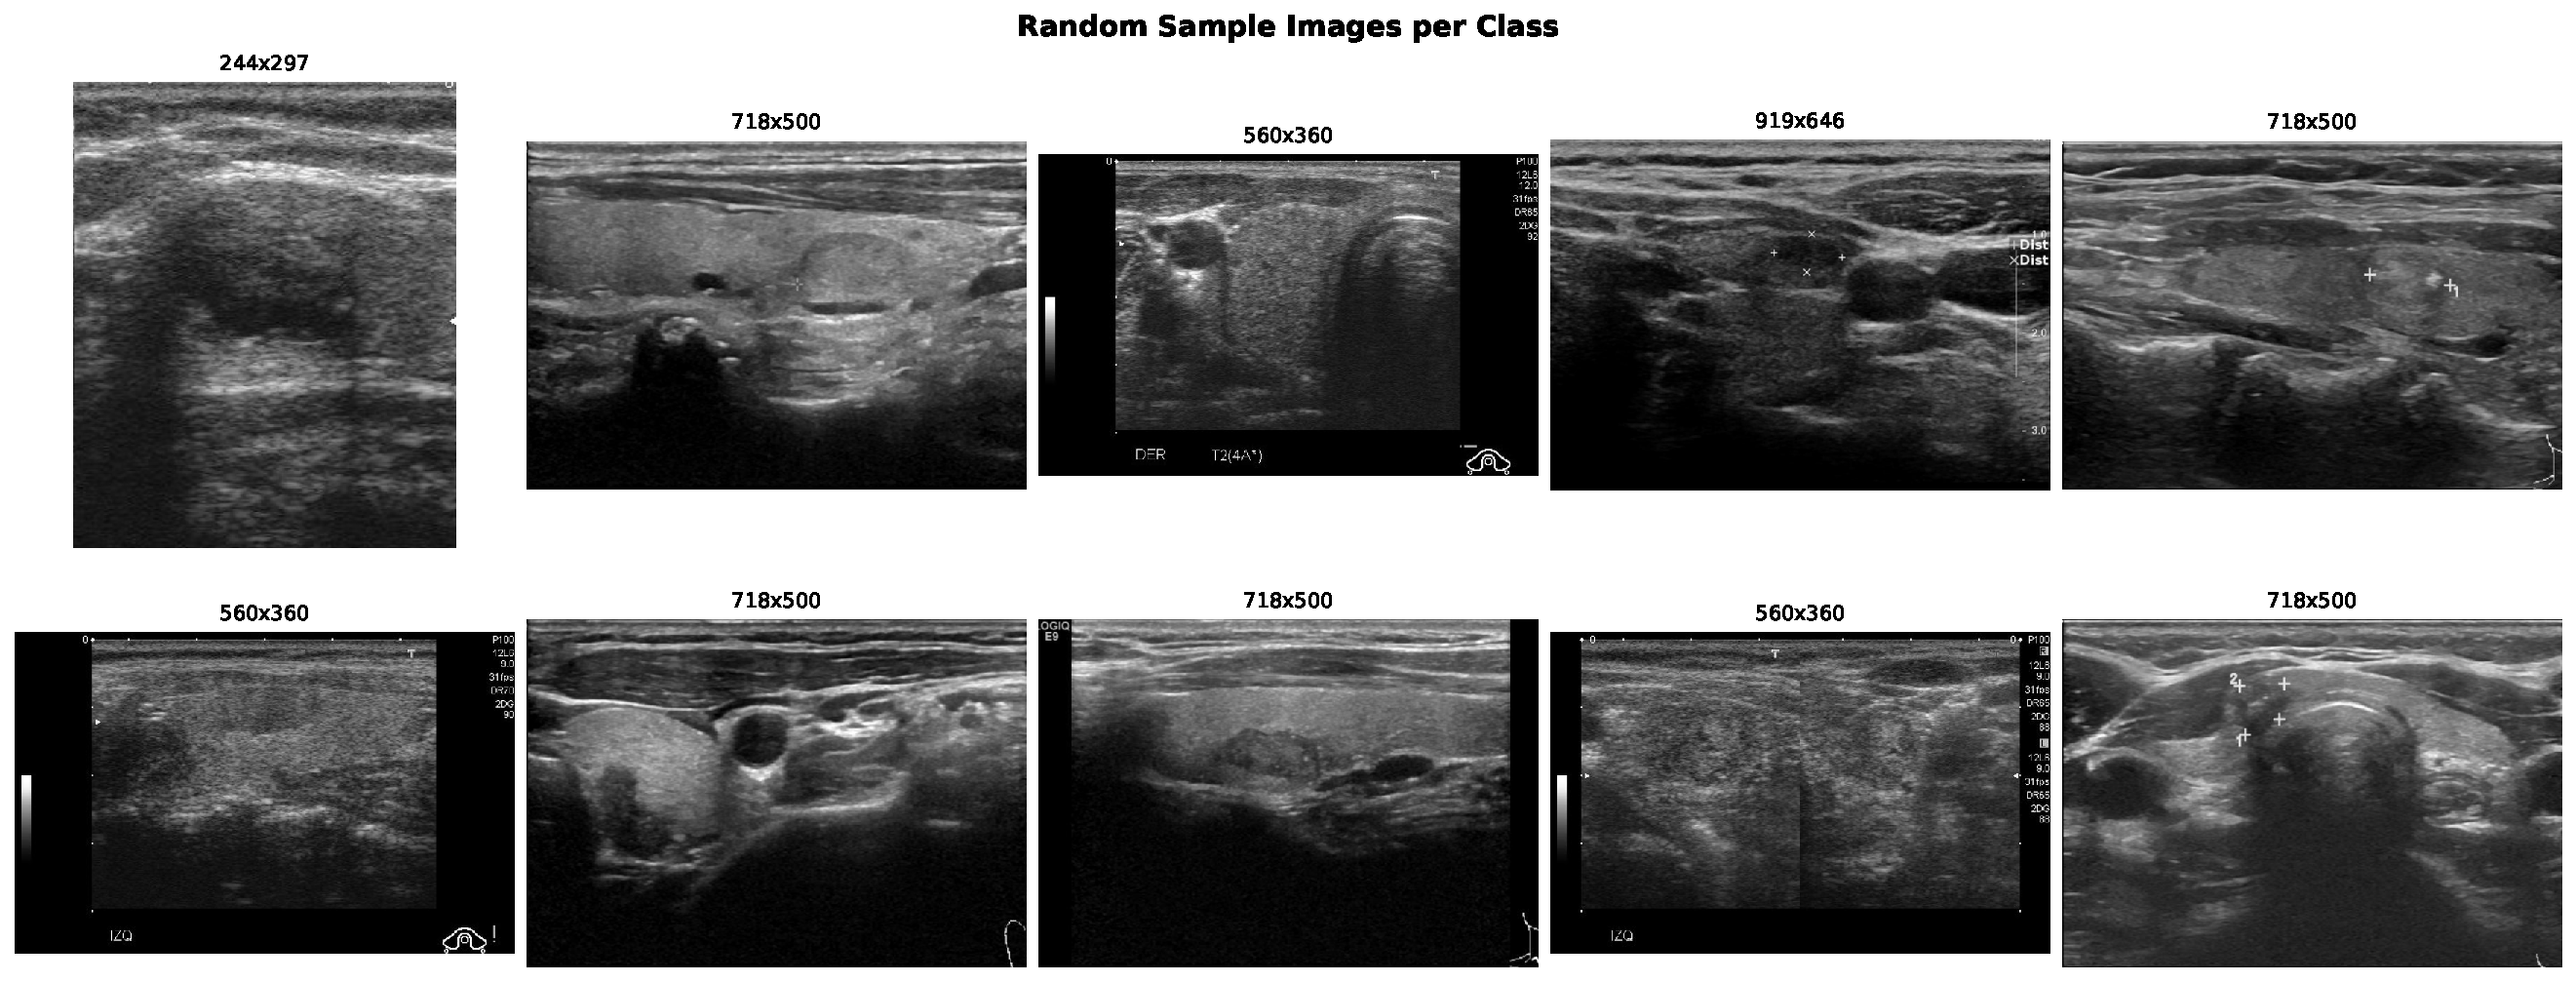
\includegraphics[width=\textwidth]{sample_images.pdf}
  \caption{Random sample images per class, showing heterogeneous resolutions and ultrasound machine overlays.}
  \label{fig:sample_images}
\end{figure*}

\subsection{Image Size Distribution}

\medskip
As shown in Fig.~\ref{fig:size_dist}, image resolutions vary widely (widths 200--1,200\,px,
heights 200--800\,px), but both classes share similar image size distribution, confirming that
size is not a decisive factor. Thus, we have decided to resize all images to a uniform scale of
$512 \times 512$.

\begin{figure*}[t]
  \centering
  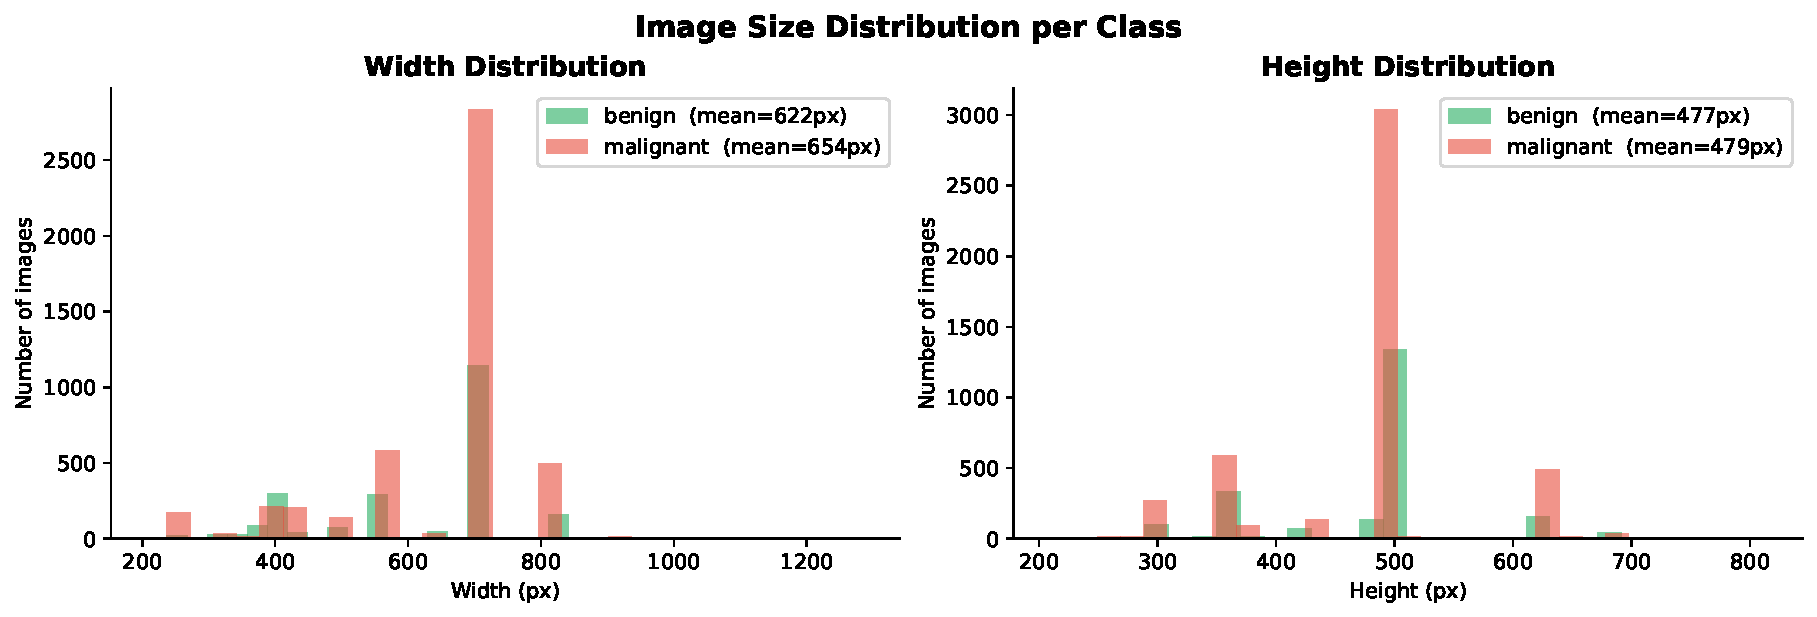
\includegraphics[width=\textwidth]{size_distribution.pdf}
  \caption{Distribution of image widths and heights per class.}
  \label{fig:size_dist}
\end{figure*}

\subsection{Domain Gap with ImageNet}

\medskip
As shown in Fig.~\ref{fig:imagenet_stats}, the dataset's per-channel means
($\approx 0.23$) are roughly half ImageNet's ($\approx 0.49$) and standard
deviations are 13--17\% lower, reflecting the dark, low-contrast nature of
ultrasound. This domain gap makes the fine-tuning strategy critical for adapting
pretrained features to this modality.

\begin{figure*}[t]
  \centering
  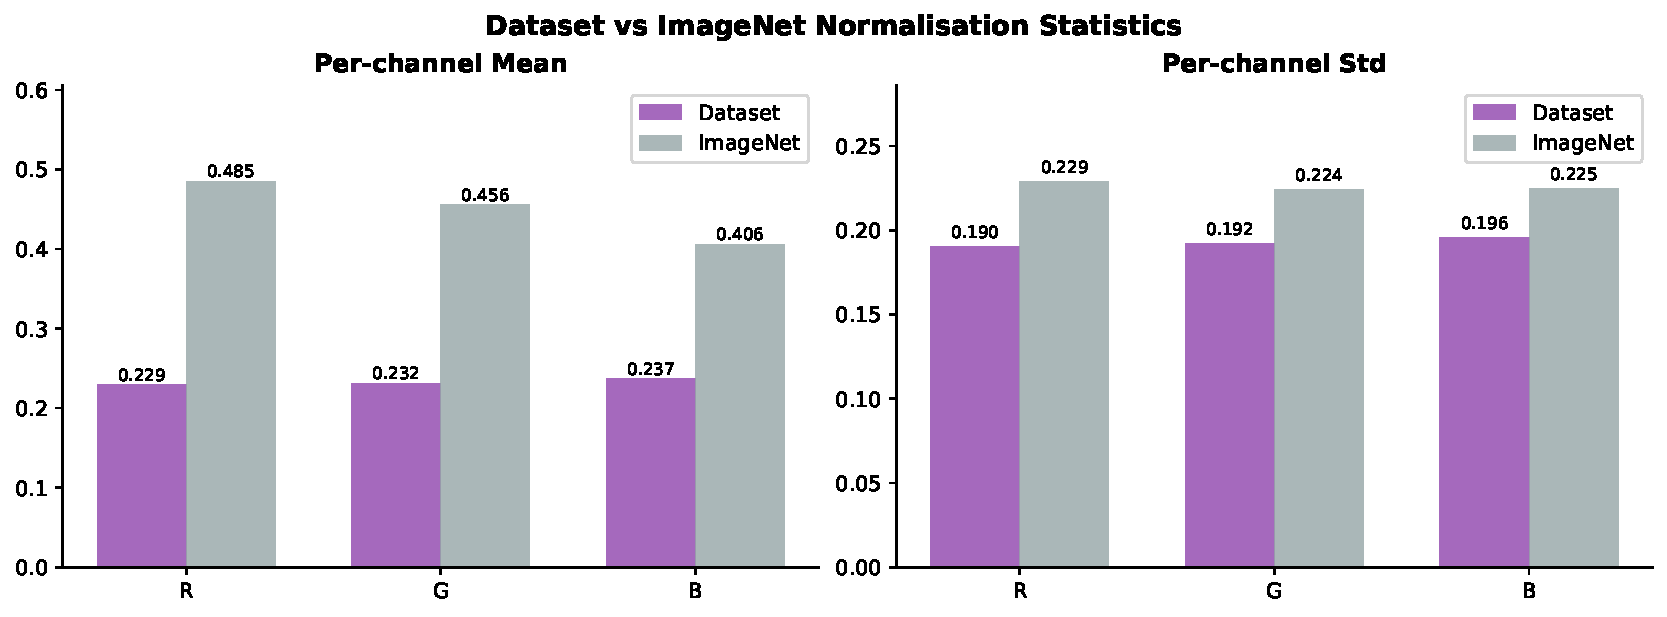
\includegraphics[width=\textwidth]{imagenet_vs_dataset.pdf}
  \caption{Per-channel normalization statistics: thyroid ultrasound dataset vs.\ ImageNet.}
  \label{fig:imagenet_stats}
\end{figure*}


\section{Methodology}

\subsection{Framework Overview}

\medskip
The proposed framework follows an end-to-end classification pipeline, as illustrated in
Fig.~\ref{fig:framework}. Raw ultrasound images are first loaded and split into stratified
train, validation, and test sets. During training, images pass through an augmentation stage
before being fed into one of three pretrained CNN backbones. The backbone is taken from
pretrained model weights, then swap the classification head, then fully unfrozen for fine-tuning
with a reduced backbone learning rate. At inference time, Test-Time Augmentation (TTA) combines
predictions across five augmented views. Then Grad-CAM heatmaps are generated after to
visualize the important regions driving each prediction.

\begin{figure}[t]
  \centering
  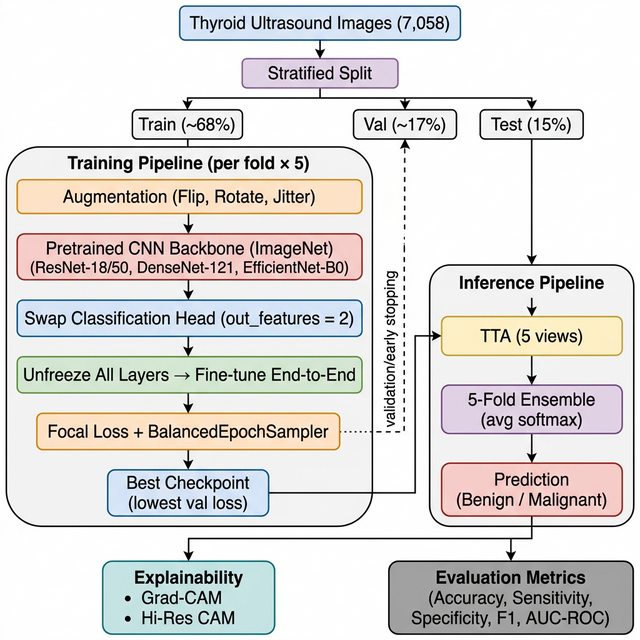
\includegraphics[width=\columnwidth]{framework_pipeline.png}
  \caption{Overview of the proposed classification framework.}
  \label{fig:framework}
\end{figure}

\subsection{Data Preprocessing}

\subsubsection{Splitting Strategy}

\medskip
To ensure reproducible and unbiased evaluation, the data is partitioned using a two-stage
stratified splitting procedure:

\begin{enumerate}
  \item \textbf{Test set}: 15\% of the full dataset is held out first as a shared test set, identical across all folds.
  \item \textbf{5-fold cross-validation}: The remaining 85\% (train + validation pool) is split using \texttt{StratifiedKFold}(\texttt{n\_splits=5}). In each fold, 4/5 of the pool is used for training and 1/5 for validation.
\end{enumerate}

This design ensures that (a) the test set is never seen during training or validation, and (b)
every sample in the train+val pool serves as a validation sample in exactly one fold. The
per-class distribution across splits is summarized in Table~\ref{tab:split_table}.

\begin{table}[t]
  \caption{Stratified data splits with per-class counts}
  \label{tab:split_table}
  \centering
  \begin{tabular}{lccc}
    \toprule
    \textbf{Split} & \textbf{Benign} & \textbf{Malignant} & \textbf{Total} \\
    \midrule
    Train ($\sim$68\%)      & 1,549 & 3,250 & 4,799 \\
    Validation ($\sim$17\%) & 387   & 813   & 1,200 \\
    Test ($\sim$15\%)       & 342   & 717   & 1,059 \\
    \midrule
    \textbf{Total}          & \textbf{2,278} & \textbf{4,780} & \textbf{7,058} \\
    \bottomrule
  \end{tabular}
\end{table}

Stratification preserves the original class ratio across all three subsets. The test set
remains fixed and shared across all cross-validation folds, ensuring a fair and consistent
final evaluation.

\subsubsection{Image Preprocessing and Augmentation}

\medskip
All images are resized to $512 \times 512$ pixels and normalized using ImageNet statistics
($\mu = [0.485, 0.456, 0.406]$, $\sigma = [0.229, 0.224, 0.225]$), which is standard practice
when using pretrained backbones.

Training augmentations are applied online to improve generalization and reduce overfitting. The
augmentation pipeline is summarized in Table~\ref{tab:aug_table}.

\begin{table}[t]
  \caption{Training augmentation configuration}
  \label{tab:aug_table}
  \centering
  \begin{tabular}{ll}
    \toprule
    \textbf{Augmentation} & \textbf{Details} \\
    \midrule
    Random Horizontal Flip & $p = 0.5$ \\
    Random Vertical Flip   & $p = 0.5$ \\
    Random Rotation        & $\pm 15^{\circ}$ \\
    Color Jitter           & brightness, contrast, saturation, hue ($\pm 0.2$) \\
    \bottomrule
  \end{tabular}
\end{table}

Validation and test transforms consist only of resizing and normalization (no augmentation),
ensuring that evaluation reflects true model performance.

\subsection{Model Architectures and Training Configuration}

\medskip
\subsubsection{Transfer Learning with Pretrained Backbones}

\medskip
All four models follow the same adaptation pattern: a pretrained ImageNet backbone is loaded
from \texttt{torchvision.models}, and the final classification head is replaced with a
\texttt{Linear}($\text{in\_features} \rightarrow 2$) layer for binary classification. The
entire network is then fine-tuned end-to-end. Table~\ref{tab:model_table} summarizes the
architectures evaluated.

\begin{table}[t]
  \caption{Summary of CNN backbones evaluated}
  \label{tab:model_table}
  \centering
  \begin{tabular}{lcc}
    \toprule
    \textbf{Backbone} & \textbf{Head in\_features} & \textbf{Approx.\ Parameters} \\
    \midrule
    ResNet-18       & 512   & $\sim$11.18M \\
    ResNet-50       & 2,048 & $\sim$23.51M \\
    DenseNet-121    & 1,024 & $\sim$6.96M  \\
    EfficientNet-B0 & 1,280 & $\sim$4.01M  \\
    \bottomrule
  \end{tabular}
\end{table}

These architectures were selected to span a range of model complexity and capacity. ResNet
variants employ residual skip connections for stable gradient flow; DenseNet-121 uses dense
connectivity to encourage feature reuse; and EfficientNet-B0 applies compound scaling to
balance depth, width, and resolution efficiently. All four have demonstrated strong performance
in medical imaging tasks.

\subsubsection{Training Hyperparameters}

\medskip
The training configuration is shared across all models and folds. For each of the 5 folds, a
fresh model with pretrained weights is initialized. The checkpoint with the lowest validation
loss is saved and used for downstream evaluation. Detailed hyperparameters are listed in
Table~\ref{tab:train_params}.

\begin{table}[t]
  \caption{Training hyperparameters}
  \label{tab:train_params}
  \centering
  \begin{tabular}{ll}
    \toprule
    \textbf{Hyperparameter} & \textbf{Value} \\
    \midrule
    Optimizer                   & Adam \\
    Learning rate               & $1 \times 10^{-4}$ \\
    Weight decay                & $1 \times 10^{-4}$ \\
    Scheduler                   & CosineAnnealingLR \\
    Epochs                      & 20 \\
    Batch size                  & 16 \\
    Early stopping patience     & 7 epochs \\
    Mixed precision (AMP)       & Enabled \\
    Number of folds             & 5 \\
    \bottomrule
  \end{tabular}
\end{table}

\subsubsection{Class Imbalance Handling}

\medskip
Two complementary strategies are applied at different levels to address the 2:1 class
imbalance:

\textbf{Sampling level --- BalancedEpochSampler.} At each epoch, \textit{all}
minority-class (benign) samples are included, and an equal number of majority-class
(malignant) samples are randomly drawn. The majority subset is reshuffled every epoch,
ensuring the model sees diverse majority-class examples across epochs while training on
balanced batches.

\textbf{Loss level --- Focal Loss.} Focal Loss~\cite{Lin2017Focal} extends standard
cross-entropy by adding a modulating factor $(1 - p_t)^{\gamma}$, where $p_t$ is the
model's estimated probability for the correct class. When the model is confident
($p_t \rightarrow 1$), this factor shrinks toward zero, effectively suppressing the loss for
easy examples. When the model is uncertain ($p_t \rightarrow 0$), the factor remains close to
1, preserving the full loss signal. The formulation is:

\begin{equation}
  \mathrm{FL}(p_t) = -\alpha \cdot (1 - p_t)^{\gamma} \cdot \log(p_t)
\end{equation}

where $\gamma = 2.0$ controls the focusing strength and $\alpha = 0.25$ balances the
contribution of each class. Using both strategies together addresses imbalance from two
complementary angles: the sampler ensures balanced data composition, while the loss function
ensures balanced gradient contribution.

\subsection{Inference Strategy}

\subsubsection{Test-Time Augmentation (TTA)}

At inference time, each input image is transformed into 5 deterministic views to reduce
prediction variance. The views are summarized in Table~\ref{tab:tta_table}.

\begin{table}[t]
  \caption{Test-Time Augmentation views}
  \label{tab:tta_table}
  \centering
  \begin{tabular}{ll}
    \toprule
    \textbf{View} & \textbf{Transformation} \\
    \midrule
    1 & Original (identity) \\
    2 & Horizontal flip \\
    3 & Vertical flip \\
    4 & Rotation $+10^{\circ}$ \\
    5 & Rotation $-10^{\circ}$ \\
    \bottomrule
  \end{tabular}
\end{table}

Each view is passed through the model independently, and the resulting softmax probabilities
are averaged to produce the final prediction for that model. This averaging smooths out
orientation-dependent biases inherent in ultrasound image acquisition.

\subsubsection{5-Fold Ensemble}

\medskip
After TTA, the averaged softmax probabilities from all 5 fold models are further averaged, and
the final class is determined by argmax. This results in $5 \times 5 = 25$ forward passes per
image (5 folds $\times$ 5 TTA views), yielding robust probabilistic predictions that reduce
the variance of any single model or single augmented view.

\subsection{Explainability: Class Activation}

\medskip
Model interpretability is critical in medical imaging --- clinicians need to understand
\textit{why} a model makes a particular prediction before trusting it in clinical workflows. We
employ two complementary Class Activation Mapping techniques to highlight the image regions
most influential to the model's decision.

\subsubsection{Grad-CAM}

\medskip
Grad-CAM~\cite{Selvaraju2017GradCAM} (Gradient-weighted Class Activation Mapping) produces
coarse localization maps by computing importance weights via Global Average Pooling (GAP) of
the gradients flowing into a target convolutional layer:

\begin{equation}
  w_k = \mathrm{GAP}\!\left(\frac{\partial y^c}{\partial A^k}\right)
\end{equation}

\begin{equation}
  \mathrm{CAM} = \mathrm{ReLU}\!\left(\sum_k w_k \cdot A^k\right)
\end{equation}

where $A^k$ denotes the $k$-th feature map from the target layer and $y^c$ is the score for
the target class $c$. The ReLU ensures that only features with a positive influence on the
prediction are retained.

\subsubsection{Hi-Res CAM}

\medskip
Hi-Res CAM~\cite{Draelos2021HiResCAM} preserves finer spatial detail by using element-wise
multiplication of gradients and activations instead of channel-level weighting:

\begin{equation}
  \mathrm{CAM} = \mathrm{ReLU}\!\left(\sum_k \nabla A^k \odot A^k\right)
\end{equation}

This produces finer-grained heatmaps compared to Grad-CAM, revealing subtle spatial patterns
that may be clinically relevant for distinguishing benign from malignant nodules.

\subsubsection{Ensemble Heatmaps}

\medskip
For each architecture, the last convolutional block is used as the target layer, as it captures
the highest-level semantic features before classification. To reduce fold-specific noise,
per-fold heatmaps are normalized to $[0, 1]$ and averaged across all 5 folds, producing stable
ensemble visualizations that reflect the consensus attention of the model.

\subsection{Evaluation Metrics}

\medskip
Model performance is evaluated on the held-out test set using the ensemble predictions. The
following standard classification metrics are adopted:

\begin{equation}
  \mathrm{Accuracy} = \frac{TP + TN}{TP + TN + FP + FN}
\end{equation}

\begin{equation}
  \mathrm{Sensitivity\,(Recall)} = \frac{TP}{TP + FN}
\end{equation}

\begin{equation}
  \mathrm{Specificity} = \frac{TN}{TN + FP}
\end{equation}

\begin{equation}
  \mathrm{Precision} = \frac{TP}{TP + FP}
\end{equation}

\begin{equation}
  F_1 = 2 \times \frac{\mathrm{Precision} \times \mathrm{Recall}}{\mathrm{Precision} + \mathrm{Recall}}
\end{equation}

where $TP$, $TN$, $FP$, and $FN$ denote True Positives, True Negatives, False Positives, and
False Negatives, respectively.

In addition, the \textbf{Area Under the ROC Curve (AUC-ROC)} is computed to measure the
model's discriminative ability across all classification thresholds. Higher AUC values indicate
better separation between benign and malignant classes.

Results are visualized through confusion matrices and ROC curves. All metrics are reported as
\textbf{mean $\pm$ standard deviation} across the 5 folds to reflect model stability, alongside
a final ensemble metric computed from the averaged predictions.

\textbf{Stacking ensemble.} As an additional baseline, a stacking meta-learner using
Logistic Regression is trained on the out-of-fold softmax probability vectors of all four
backbone models. The meta-learner is fitted on the validation folds and evaluated on the
held-out test set using the same metrics above.


\section{Evaluation Results}

\subsection{Models Performance Comparison}

Several state-of-the-art methods, such as Hybrid CNN~\cite{bahmane2025hybrid} and Vision
Transformer (ViT) approaches~\cite{sujini2025automated}, achieve high accuracy by using
GAN-based augmentation to generate synthetic images for addressing class imbalance. In contrast,
our approach prioritizes medical reliability by training exclusively on real ultrasound images.
Notably, our DenseNet-121 model~\cite{Huang2017DenseNet} achieves a strong AUC of 93.76\%,
outperforming both Hybrid CNN (91.00\%)~\cite{bahmane2025hybrid} and ROI + Context GNN
(90.60\%)~\cite{yavuz2026roi}.

AUC is particularly important in medical diagnosis because it measures the model's ability to
distinguish malignant from benign cases across multiple thresholds.

\begin{table}[h!]
  \caption{Performance comparison of our models against state-of-the-art methods}
  \label{tab:perf_compare}
  \centering
  \footnotesize
  \setlength{\tabcolsep}{4pt}
  \begin{tabular}{lccccc}
    \toprule
    \textbf{Model} & \textbf{Acc.} & \textbf{Sens.} & \textbf{Spec.} & \textbf{F1} & \textbf{AUC} \\
    \midrule
    \multicolumn{6}{l}{\textit{Our Implemented Models}} \\
    \midrule
    ResNet-18                      & 86.50\% & 88.01\% & 83.33\% & 86.83\% & 93.15\% \\
    ResNet-50                      & 85.17\% & 88.98\% & 77.19\%          & 85.18\% & 92.82\% \\
    DenseNet-121                   & \textbf{87.35\%} & \textbf{89.96\%} & 81.87\% & \textbf{87.39\%} & \textbf{93.76\%} \\
    EfficientNet-B0                & 85.84\% & 87.03\% & 83.33\% & 86.01\% & 92.38\% \\
    Stacking (LR)                  & 85.70\% & 85.36\% & \textbf{85.09\%}          & 85.52\% & 93.55\% \\
    \midrule
    \multicolumn{6}{l}{\textit{Related Works (TN5000)}} \\
    \midrule
    Hybrid CNN~\cite{bahmane2025hybrid}        & 89.73\% & 90.01\% & 88.70\% & 88.85\% & 91.60\% \\
    ROI+Context GNN~\cite{yavuz2026roi}        & 90.40\% & ---     & ---     & 92.20\% & 90.60\% \\
    ViT+WGAN-GP~\cite{sujini2025automated}     & 96.80\% & 97.30\% & 96.40\% & 96.50\% & 98.60\% \\
    \bottomrule
  \end{tabular}
\end{table}

\subsection{Confusion Matrix}

\begin{figure}[H]
  \centering
  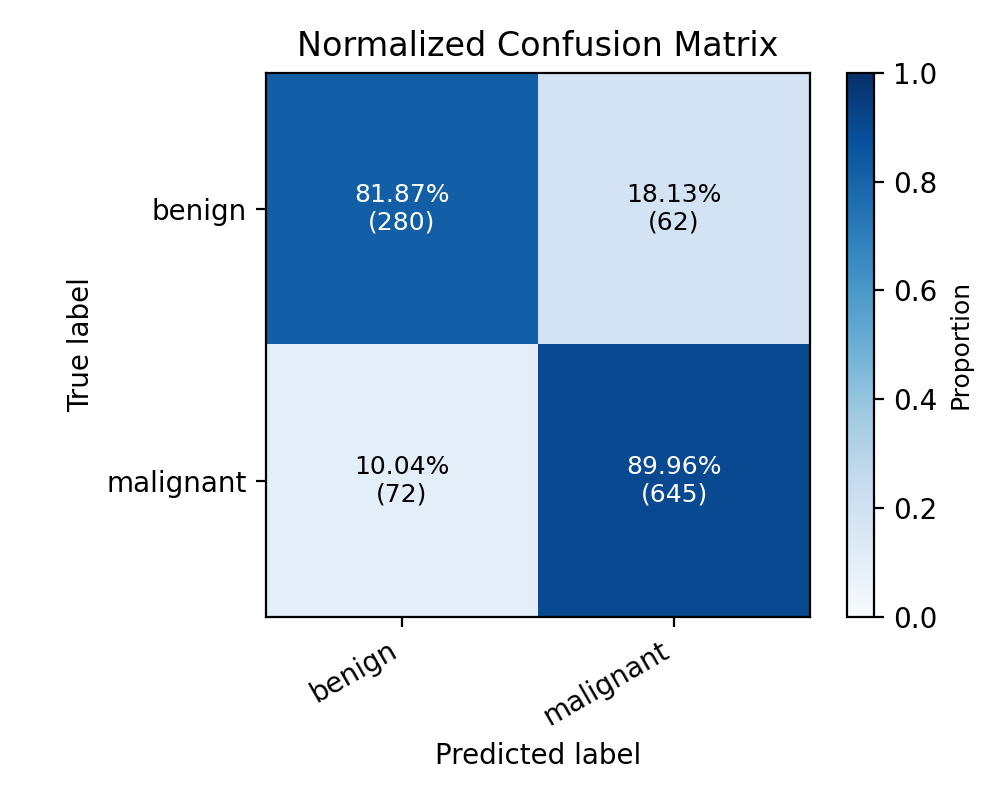
\includegraphics[width=1.07\columnwidth]{conf_matrix3.png}
  \caption{Confusion matrix for DenseNet-121.}
  \label{fig:conf_matrix_densenet}
\end{figure}

\subsection{ROC Curves Analysis}

\begin{figure}[H]
  \centering
  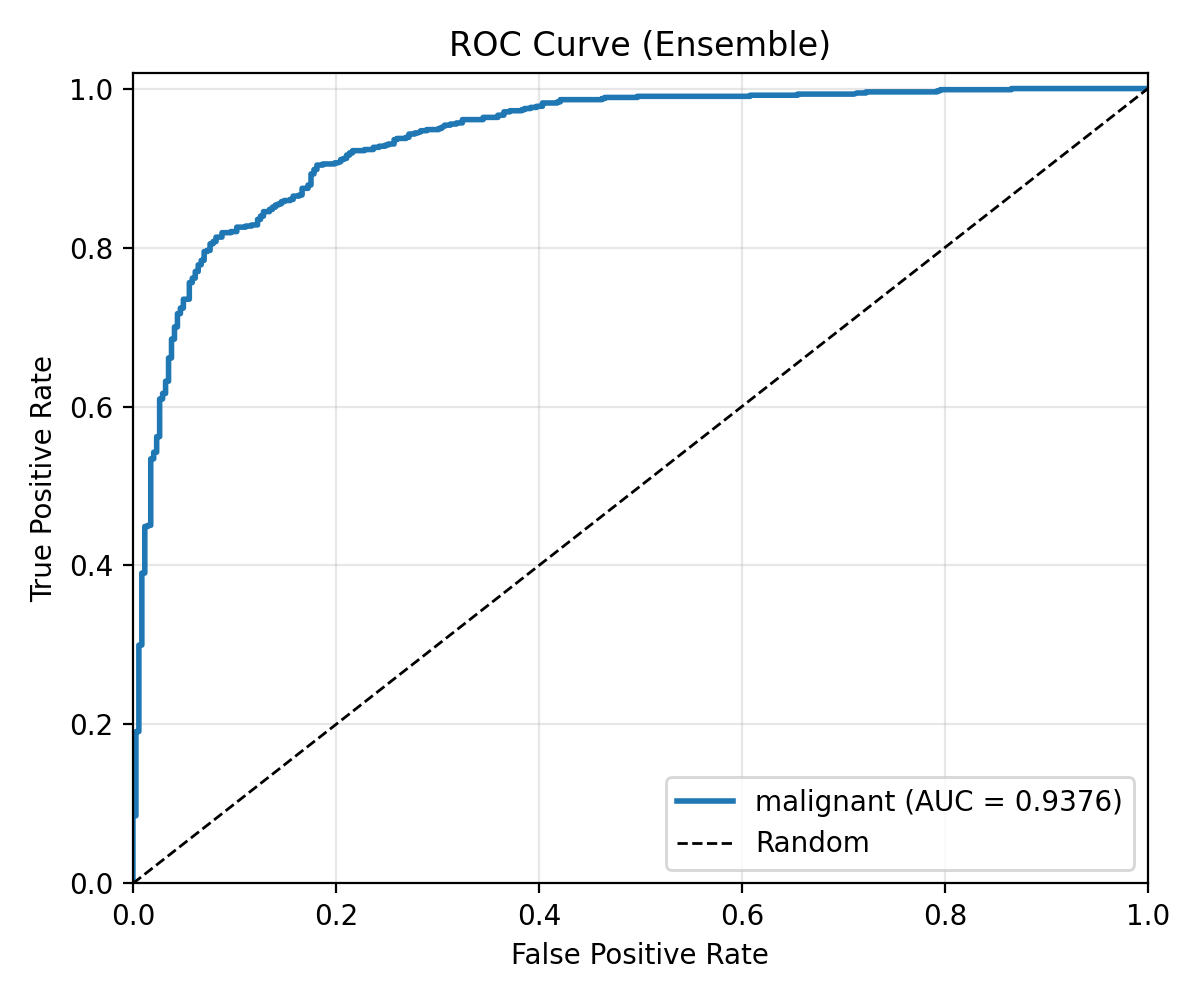
\includegraphics[width=\columnwidth]{ROC3.png}
  \caption{ROC Curve for DenseNet-121.}
  \label{fig:roc_densenet}
\end{figure}


\section{Conclusion and Future Works}

In this project, we have successfully developed and evaluated an end-to-end deep learning
framework for binary thyroid ultrasound classification. By fine-tuning four pretrained CNN
backbones which are ResNet-18, ResNet-50, DenseNet-121, and EfficientNet-B0 with a carefully
designed training pipeline, our models can achieve high classification results.

These results suggest that our training pipeline using Mixup augmentation~\cite{Zhang2018Mixup},
Focal Loss~\cite{Lin2017Focal} and Test-Time Augmentation (TTA) effectively captures diagnostic
features from real ultrasound images without relying on complex graph-based
architectures~\cite{yavuz2026roi} or potentially unreliable synthetic image
generation~\cite{sujini2025automated}.

Beyond classification accuracy, we incorporated Grad-CAM and Hi-Res CAM visualizations to
provide interpretable evidence for model decisions, more specifically, they will highlight
regions that is important for model's decision for classification of images that contain
malignant tumor.

We additionally implemented a stacking ensemble using Logistic Regression as a meta-learner
on the out-of-fold predictions of all four backbones, achieving an AUC of 93.55\% and
improving specificity to 85.09\%, demonstrating the benefit of combining diverse architectures.

Future work includes model compression (quantization and pruning) for deployment on portable
ultrasound devices, specificity-oriented training via cost-sensitive learning and threshold
calibration to reduce unnecessary FNA biopsies, and extension to video-based classification
using spatiotemporal models such as 3D-CNNs or ConvLSTMs.


\bibliographystyle{IEEEtran}
\bibliography{refs}


\appendix

\begin{figure*}[!t]
  \centering
  \includegraphics[width=0.75\textwidth]{compare_cam_densenet1.png}
\end{figure*}

\begin{figure*}[!t]
  \centering
  % Left column: Confusion matrices
  \begin{minipage}[t]{0.48\textwidth}
    \begin{subfigure}[t]{\textwidth}
      \centering
      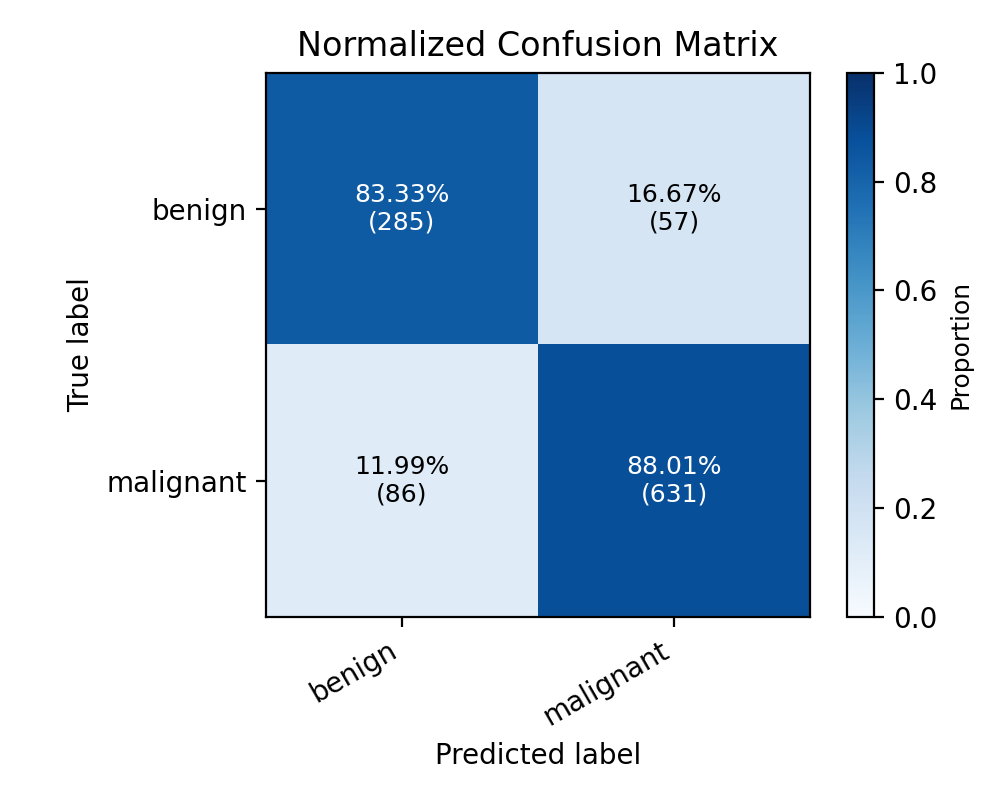
\includegraphics[width=\textwidth]{conf_matrix1.png}
      \caption{Confusion matrix for ResNet-18.}
    \end{subfigure}
    \vspace{0.4em}
    \begin{subfigure}[t]{\textwidth}
      \centering
      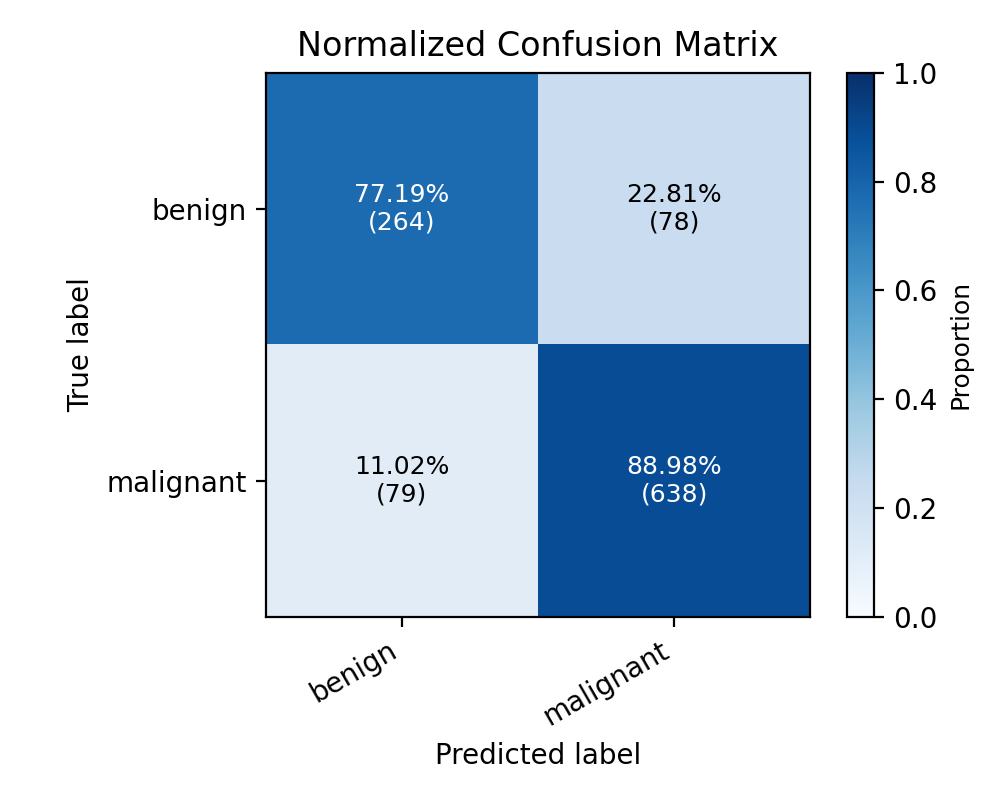
\includegraphics[width=\textwidth]{conf_matrix2.png}
      \caption{Confusion matrix for ResNet-50.}
    \end{subfigure}
    \vspace{0.4em}
    \begin{subfigure}[t]{\textwidth}
      \centering
      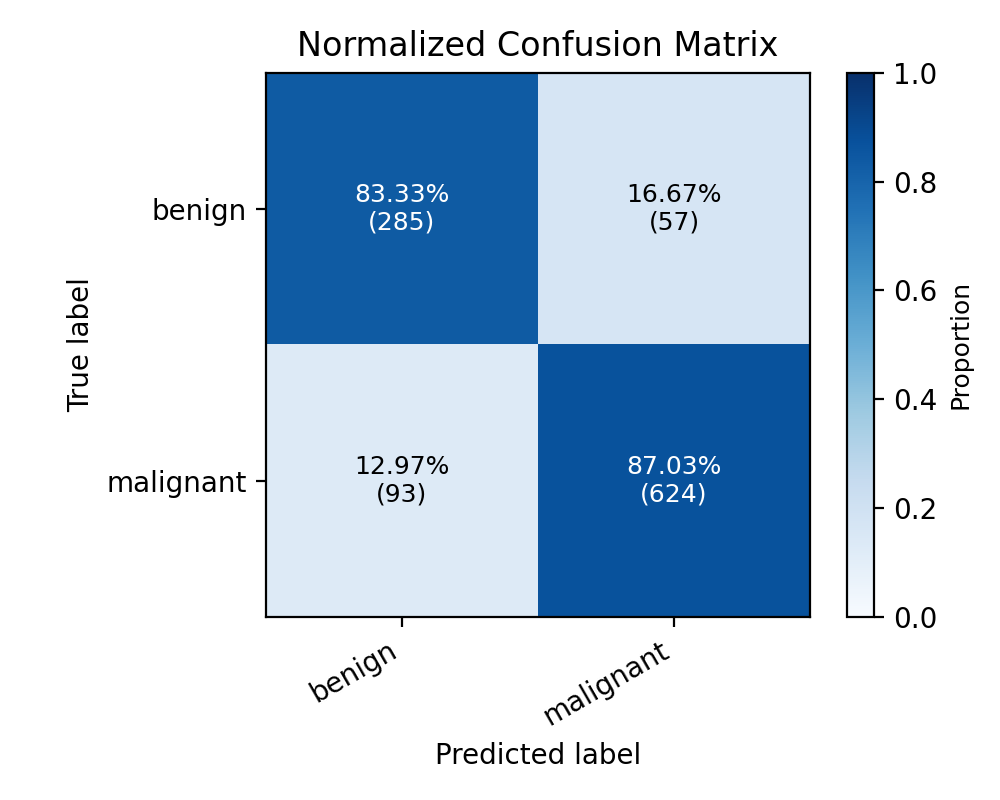
\includegraphics[width=\textwidth]{conf_matrix4.png}
      \caption{Confusion matrix for EfficientNet-B0.}
    \end{subfigure}
  \end{minipage}
  \hfill
  % Right column: ROC curves
  \begin{minipage}[t]{0.48\textwidth}
    \begin{subfigure}[t]{\textwidth}
      \centering
      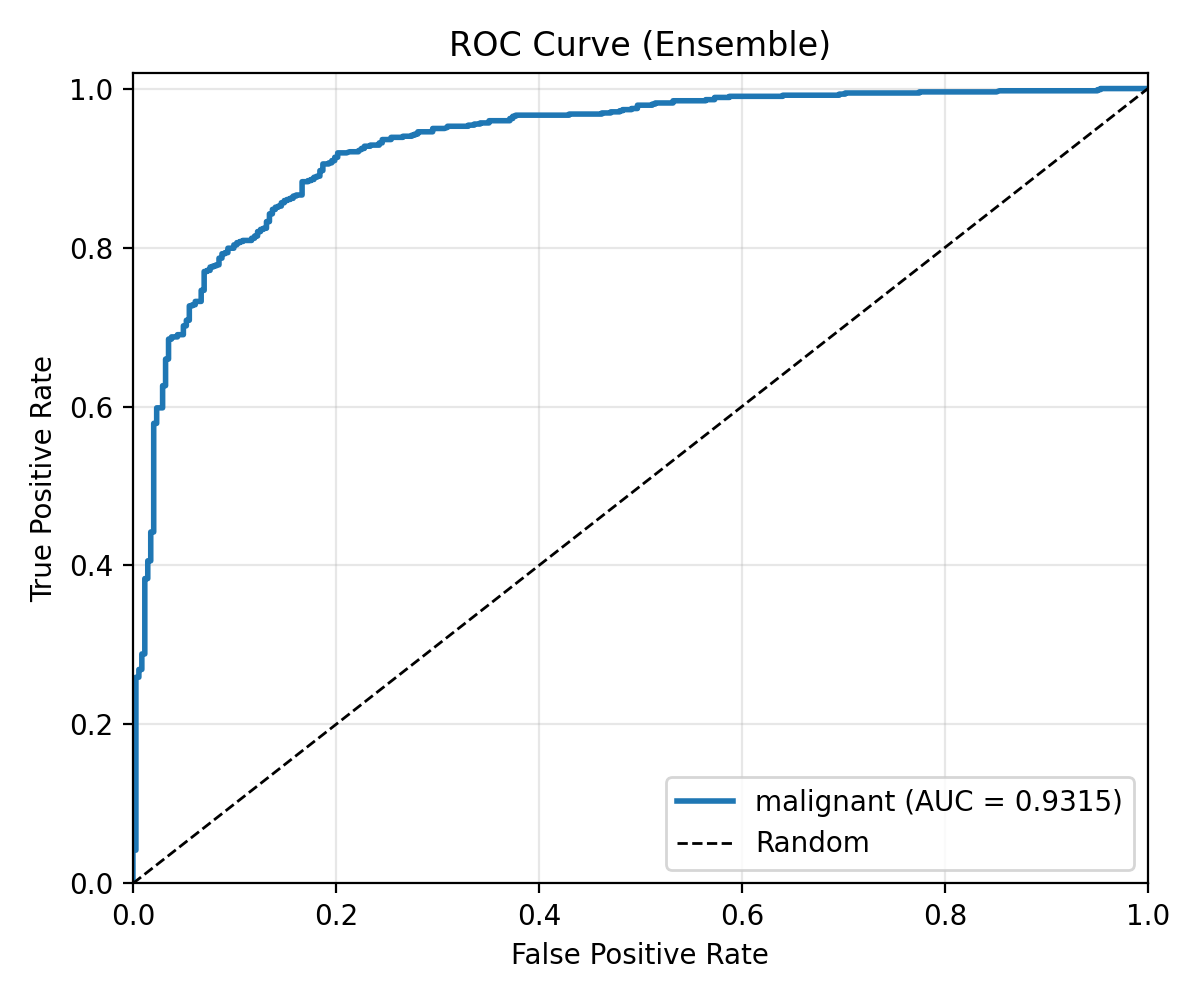
\includegraphics[width=\textwidth]{ROC1.png}
      \caption{ROC Curve for ResNet-18.}
    \end{subfigure}
    \vspace{0.4em}
    \begin{subfigure}[t]{\textwidth}
      \centering
      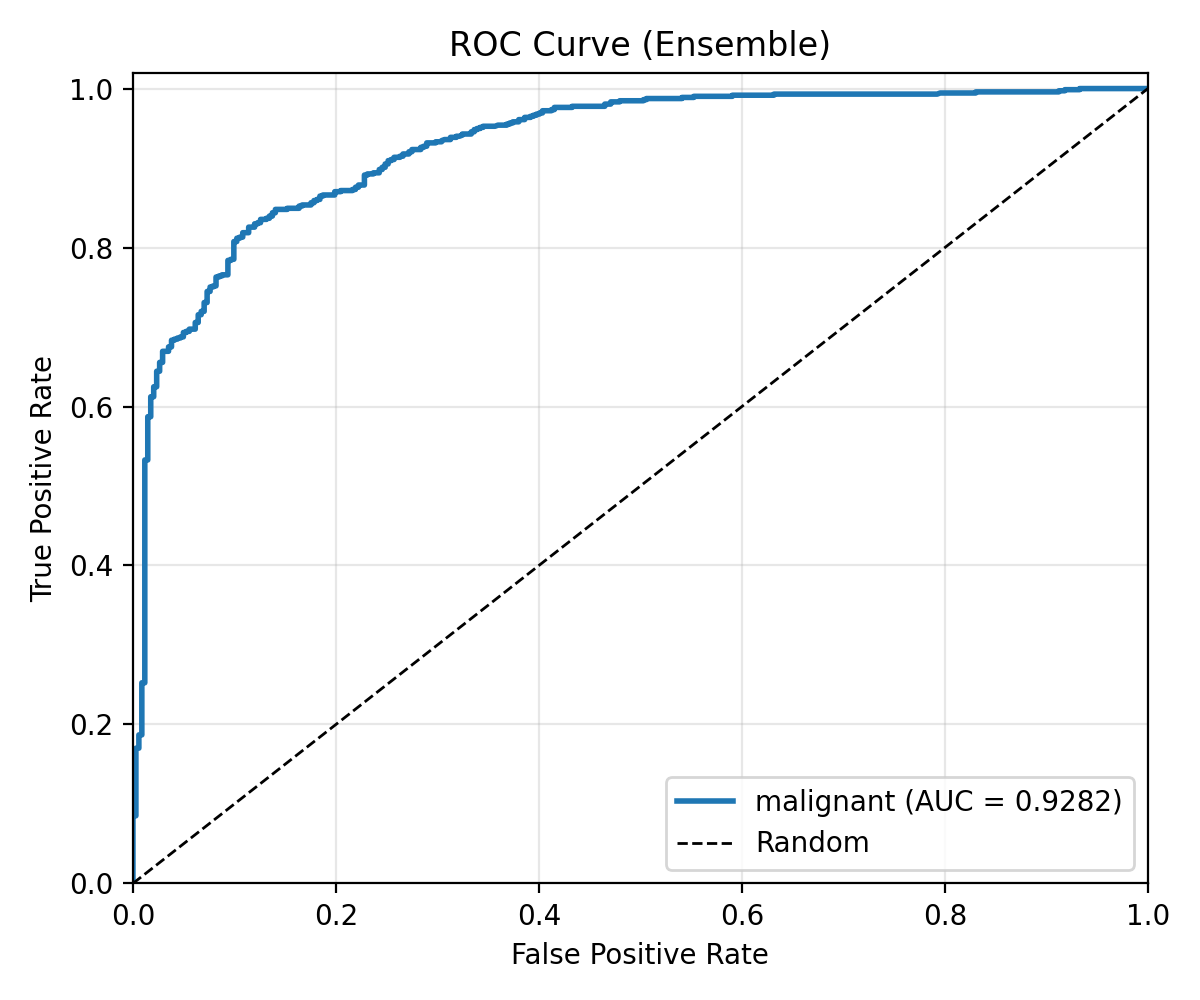
\includegraphics[width=\textwidth]{ROC2.png}
      \caption{ROC Curve for ResNet-50.}
    \end{subfigure}
    \vspace{0.4em}
    \begin{subfigure}[t]{\textwidth}
      \centering
      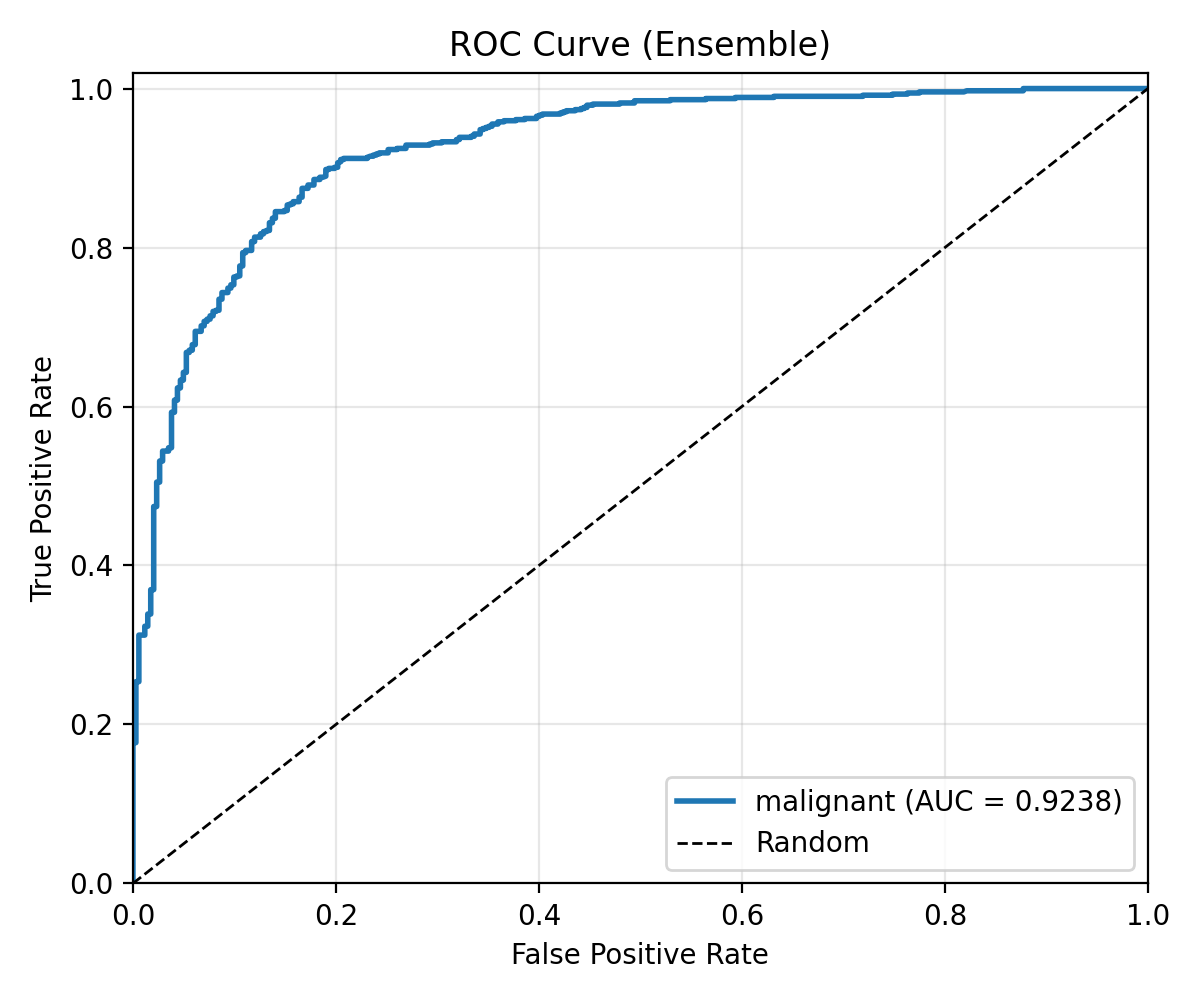
\includegraphics[width=\textwidth]{ROC4.png}
      \caption{ROC Curve for EfficientNet-B0.}
    \end{subfigure}
  \end{minipage}
  \caption{Confusion matrices (left) and ROC curves (right) for ResNet-18, ResNet-50, and EfficientNet-B0.}
\end{figure*}

\end{document}
